% Options for packages loaded elsewhere
\PassOptionsToPackage{unicode}{hyperref}
\PassOptionsToPackage{hyphens}{url}
\PassOptionsToPackage{dvipsnames,svgnames,x11names}{xcolor}
%
\documentclass[
  letterpaper,
  DIV=11,
  numbers=noendperiod]{scrartcl}

\usepackage{amsmath,amssymb}
\usepackage{iftex}
\ifPDFTeX
  \usepackage[T1]{fontenc}
  \usepackage[utf8]{inputenc}
  \usepackage{textcomp} % provide euro and other symbols
\else % if luatex or xetex
  \usepackage{unicode-math}
  \defaultfontfeatures{Scale=MatchLowercase}
  \defaultfontfeatures[\rmfamily]{Ligatures=TeX,Scale=1}
\fi
\usepackage{lmodern}
\ifPDFTeX\else  
    % xetex/luatex font selection
\fi
% Use upquote if available, for straight quotes in verbatim environments
\IfFileExists{upquote.sty}{\usepackage{upquote}}{}
\IfFileExists{microtype.sty}{% use microtype if available
  \usepackage[]{microtype}
  \UseMicrotypeSet[protrusion]{basicmath} % disable protrusion for tt fonts
}{}
\makeatletter
\@ifundefined{KOMAClassName}{% if non-KOMA class
  \IfFileExists{parskip.sty}{%
    \usepackage{parskip}
  }{% else
    \setlength{\parindent}{0pt}
    \setlength{\parskip}{6pt plus 2pt minus 1pt}}
}{% if KOMA class
  \KOMAoptions{parskip=half}}
\makeatother
\usepackage{xcolor}
\setlength{\emergencystretch}{3em} % prevent overfull lines
\setcounter{secnumdepth}{-\maxdimen} % remove section numbering
% Make \paragraph and \subparagraph free-standing
\makeatletter
\ifx\paragraph\undefined\else
  \let\oldparagraph\paragraph
  \renewcommand{\paragraph}{
    \@ifstar
      \xxxParagraphStar
      \xxxParagraphNoStar
  }
  \newcommand{\xxxParagraphStar}[1]{\oldparagraph*{#1}\mbox{}}
  \newcommand{\xxxParagraphNoStar}[1]{\oldparagraph{#1}\mbox{}}
\fi
\ifx\subparagraph\undefined\else
  \let\oldsubparagraph\subparagraph
  \renewcommand{\subparagraph}{
    \@ifstar
      \xxxSubParagraphStar
      \xxxSubParagraphNoStar
  }
  \newcommand{\xxxSubParagraphStar}[1]{\oldsubparagraph*{#1}\mbox{}}
  \newcommand{\xxxSubParagraphNoStar}[1]{\oldsubparagraph{#1}\mbox{}}
\fi
\makeatother


\providecommand{\tightlist}{%
  \setlength{\itemsep}{0pt}\setlength{\parskip}{0pt}}\usepackage{longtable,booktabs,array}
\usepackage{calc} % for calculating minipage widths
% Correct order of tables after \paragraph or \subparagraph
\usepackage{etoolbox}
\makeatletter
\patchcmd\longtable{\par}{\if@noskipsec\mbox{}\fi\par}{}{}
\makeatother
% Allow footnotes in longtable head/foot
\IfFileExists{footnotehyper.sty}{\usepackage{footnotehyper}}{\usepackage{footnote}}
\makesavenoteenv{longtable}
\usepackage{graphicx}
\makeatletter
\def\maxwidth{\ifdim\Gin@nat@width>\linewidth\linewidth\else\Gin@nat@width\fi}
\def\maxheight{\ifdim\Gin@nat@height>\textheight\textheight\else\Gin@nat@height\fi}
\makeatother
% Scale images if necessary, so that they will not overflow the page
% margins by default, and it is still possible to overwrite the defaults
% using explicit options in \includegraphics[width, height, ...]{}
\setkeys{Gin}{width=\maxwidth,height=\maxheight,keepaspectratio}
% Set default figure placement to htbp
\makeatletter
\def\fps@figure{htbp}
\makeatother
% definitions for citeproc citations
\NewDocumentCommand\citeproctext{}{}
\NewDocumentCommand\citeproc{mm}{%
  \begingroup\def\citeproctext{#2}\cite{#1}\endgroup}
\makeatletter
 % allow citations to break across lines
 \let\@cite@ofmt\@firstofone
 % avoid brackets around text for \cite:
 \def\@biblabel#1{}
 \def\@cite#1#2{{#1\if@tempswa , #2\fi}}
\makeatother
\newlength{\cslhangindent}
\setlength{\cslhangindent}{1.5em}
\newlength{\csllabelwidth}
\setlength{\csllabelwidth}{3em}
\newenvironment{CSLReferences}[2] % #1 hanging-indent, #2 entry-spacing
 {\begin{list}{}{%
  \setlength{\itemindent}{0pt}
  \setlength{\leftmargin}{0pt}
  \setlength{\parsep}{0pt}
  % turn on hanging indent if param 1 is 1
  \ifodd #1
   \setlength{\leftmargin}{\cslhangindent}
   \setlength{\itemindent}{-1\cslhangindent}
  \fi
  % set entry spacing
  \setlength{\itemsep}{#2\baselineskip}}}
 {\end{list}}
\usepackage{calc}
\newcommand{\CSLBlock}[1]{\hfill\break\parbox[t]{\linewidth}{\strut\ignorespaces#1\strut}}
\newcommand{\CSLLeftMargin}[1]{\parbox[t]{\csllabelwidth}{\strut#1\strut}}
\newcommand{\CSLRightInline}[1]{\parbox[t]{\linewidth - \csllabelwidth}{\strut#1\strut}}
\newcommand{\CSLIndent}[1]{\hspace{\cslhangindent}#1}

\KOMAoption{captions}{tableheading}
\makeatletter
\@ifpackageloaded{caption}{}{\usepackage{caption}}
\AtBeginDocument{%
\ifdefined\contentsname
  \renewcommand*\contentsname{Table of contents}
\else
  \newcommand\contentsname{Table of contents}
\fi
\ifdefined\listfigurename
  \renewcommand*\listfigurename{List of Figures}
\else
  \newcommand\listfigurename{List of Figures}
\fi
\ifdefined\listtablename
  \renewcommand*\listtablename{List of Tables}
\else
  \newcommand\listtablename{List of Tables}
\fi
\ifdefined\figurename
  \renewcommand*\figurename{Figure}
\else
  \newcommand\figurename{Figure}
\fi
\ifdefined\tablename
  \renewcommand*\tablename{Table}
\else
  \newcommand\tablename{Table}
\fi
}
\@ifpackageloaded{float}{}{\usepackage{float}}
\floatstyle{ruled}
\@ifundefined{c@chapter}{\newfloat{codelisting}{h}{lop}}{\newfloat{codelisting}{h}{lop}[chapter]}
\floatname{codelisting}{Listing}
\newcommand*\listoflistings{\listof{codelisting}{List of Listings}}
\makeatother
\makeatletter
\makeatother
\makeatletter
\@ifpackageloaded{caption}{}{\usepackage{caption}}
\@ifpackageloaded{subcaption}{}{\usepackage{subcaption}}
\makeatother
\ifLuaTeX
  \usepackage{selnolig}  % disable illegal ligatures
\fi
\usepackage{bookmark}

\IfFileExists{xurl.sty}{\usepackage{xurl}}{} % add URL line breaks if available
\urlstyle{same} % disable monospaced font for URLs
\hypersetup{
  pdftitle={Investigating Shark Attack Survivability},
  colorlinks=true,
  linkcolor={blue},
  filecolor={Maroon},
  citecolor={Blue},
  urlcolor={Blue},
  pdfcreator={LaTeX via pandoc}}

\title{Investigating Shark Attack Survivability}
\usepackage{etoolbox}
\makeatletter
\providecommand{\subtitle}[1]{% add subtitle to \maketitle
  \apptocmd{\@title}{\par {\large #1 \par}}{}{}
}
\makeatother
\subtitle{DSAN 5650: Causal Inference for Computational Social Science}
\author{Ian Alvarado}
\date{2026-08-07}

\begin{document}
\maketitle
\begin{abstract}
This project aims to identify the causal relationship between several
variables and the survivability of a shark attack using data from the
Global Shark Attack File (GSAF). In particular, this study investigates
how the activity an individual chooses at the beach affects the odds of
survival in the event of a shark attack. Initial exploratory data
analysis reveals that the survivability of an attack varies dramatically
between activities such as surfing, swimming, wading, etc. The overall
fatality rate of shark attacks was found to be 15.6\%. Fatality rates of
specific activities vary dramatically, with the highest fatality rate
being swimming (26.7\%) and the lowest being stand-up paddle boarding
(2.7\%). However, this initial analysis ignores the potential impact of
several confounding variables found within the GSAF dataset. Species is
an important confounding variable, as a shark's size and behavior are
major determinants in whether an attack on a human results in death.
Given an attack, both the species and the activity of the victim are
likely influenced by the location and time of year of the attack. The
three confounding variables we focus on for this study are location,
season, and species. Further analysis reveals that the fatality rates of
attacks given different activities vary between locations, species, and
seasons. For example, the fatality rate of attacks on swimmers in
Florida is 9.1\% while the fatality rate of attacks on swimmers in New
South Wales is 48.7\%. This finding highlights the importance of
considering how those variables confound the associational effect found
between activity and survivability when examining the entire dataset.
This study then proceeds to propose a method to model the interaction
between activity, fatality, and the confounding variables using a
probabilistic graphical model. Lastly, this paper attempts to implement
this model using PyMC. This model could then be used to perform
do-calculus to isolate the causal effect of activity on fatality.
\end{abstract}

\subsection{Introduction}\label{sec-1}

The fear of shark attacks shapes the relationship many people have with
the ocean, often keeping some of them away from it entirely. Due to
their rarity, people's perception and understanding of shark attacks are
almost entirely shaped by stories and their depiction in media. This
understanding has real-life consequences for recreation at the beach.
Neff (2015) introduces the idea of the ``Jaws Effect'' and argues that
fictional depictions of shark attacks become the basis for explaining
real-life events by political actors who influence policy. The way shark
attacks are portrayed in media often suggests the intentionality of the
shark, villifying the animal. More importantly for our analysis, shark
attacks in media often reinforce the idea that encounters with sharks
lead to fatal outcomes. Our analysis in later sections will push back
against this idea, instead showing the majority of shark attacks (let
alone shark encounters) are not fatal. Nonetheless, the portrayal of
sharks as inherently evil and lethal animals shapes policy and may be
one of the reasons nearly 100 million sharks are killed by humans each
year, as detailed by Worm et al. (2013). Data analysis can unearth
findings that create a more accurate understanding of sharks and their
interactions with humans. Such an understanding could then be used by
policymakers to keep humans and sharks safer through education,
warnings, and even physical solutions such as shark nets and drone
spotters.

There is existing literature conducting a variety of analyses on the
Global Shark Attack File (GSAF), including some that focus on the
fatality rates of shark attacks. Ricci et al. (2016) examines the type
of injuries that arise from shark attacks and even goes so far as to
investigate which characteristics of an attack lead to severe injuries
and death. One such attack characteristic is the activity of the victim
at the time of the attack (identifying swimming as the most lethal
activity). Vasconcelos et al. (2021) go a step further, looking at shark
attacks in Brazil. They investigate other factors such as region,
demographic information, and even temporal variables such as time of
year. Such studies are useful. However, they do not go beyond an
associational analysis of the factors contributing to fatal shark
attacks. This paper aims to go beyond associational analysis and conduct
a causal analysis of the variables that influence the survivability of
shark attacks. Ultimately discovering which factors truly cause shark
attacks to be deadly.

This paper primarily focuses on one shark attack characteristic, the
activity of the victim at the time of attack. While Ricci et al. (2016)
and Vasconcelos et al. (2021) both identify activity as a contributing
factor to shark attack survivability, neither quantifies the causal
change in survivability by choosing to partake in one activity over
others. Activity is one of the only characteristics of an attack listed
in the GSAF that is truly a choice of the victim, and is therefore one
of the variables a potential victim would have the most control over.
Enabling people with accurate data relating to activity and shark attack
survivability would allow them to make the most informed choice while
having a nearly complete understanding of the risks associated with
their chosen activity.

\subsection{Exploratory data analysis}\label{sec-2}

Data for this project is from the Global Shark Attack File
(\href{https://www.sharkattackfile.net/incidentlog.htm}{GSAF}). The GSAF
is maintained by the Shark Research Institute and has over 5000 records
of shark attacks dating all the way back to the 17th Century. While an
invaluable resource for the study of shark attacks, there are multiple
concerns with this dataset. First and foremost is the selection bias of
what attacks actually end up recorded in this dataset. The majority of
attacks recorded in the GSAF are from the United States and Australia,
which are wealthy, populous, and developed nations. Attacks in these
countries are highly publicized and have the ability to be easily
reported through media such as print and the internet. Nations that are
less developed, particularly those in the South Pacific and the global
south as a whole, likely have a more difficult time reporting and
communicating attacks in such a way that they would ultimately end up in
the GSAF. One should assume that there is a lack of reported attacks
from less developed countries that end up in the GSAF, especially as one
looks further back in time. Other concerns exist within the dataset
itself. Many of the records in the GSAF are missing data for one or more
attributes of a given attack (e.g., missing date and/or species).
Additionally, the data itself can be quite messy. Many records contain
typos and descriptions of attributes that can be vague or
hyper-specific. This section details how the data was prepared for
subsequent analysis.

\subsubsection{Data preparation}\label{data-preparation}

The raw data was downloaded from the GSAF. This data was then cleaned
using scripts that can be found in the code folder included in the
GitHub repository that is linked at the top of this page. This cleaning
included selecting which columns to keep for analysis. Of those columns
kept, several mapped descriptive strings to categories. For example, the
script would look for keywords in the description such as ``surfing'',
``surboard'', or ``boogieboard'' and map them to the category
``surfing/bodyboarding''. A similar process was performed to turn data
in the ``state'' and ``species'' columns into categorical variables. The
resulting clean data was then filtered for records that cleanly mapped
to activities of interest and had non-null values for fatality. Lastly,
columns were added for hemisphere in order to ultimately add a column
specifying the season in which an attack occurred.

This data was then further filtered down according to geographic area.
First only the top ten countries by attack count were kept, the top 10
countries account for 79\% of all attacks recorded in the GSAF (leaving
4099 records). However, country will not work as a variable for location
by itself as it is too vague. For example, both California and Flordia
are in the United States yet have very different climates and shark
species present. This data was then further filtered down to states
(including state-like territories in other countries) in order to get
more granular location data. These states were then further filtered
down to states that had at least 30 attacks recorded in the GSAF. This
left 20 states remaining in the dataset, statistics on this cleaned and
filtered dataset can be seen below.

\begin{itemize}
\tightlist
\item
  Total number of attacks: 3358
\item
  Number of fatal attacks: 524
\item
  Number of nonfatal attacks: 2834
\item
  Overall fatality rate: 15.60\%
\end{itemize}

\subsubsection{Fatality rates by different
attributes}\label{fatality-rates-by-different-attributes}

\paragraph{Analysis of activity}\label{analysis-of-activity}

Figure 1 shows the count of shark attacks and fatality rates for
different activities. The overall fatality rate of 15.6\% is shown on
the rate visualization as a dashed red line.

\begin{figure}

\centering{

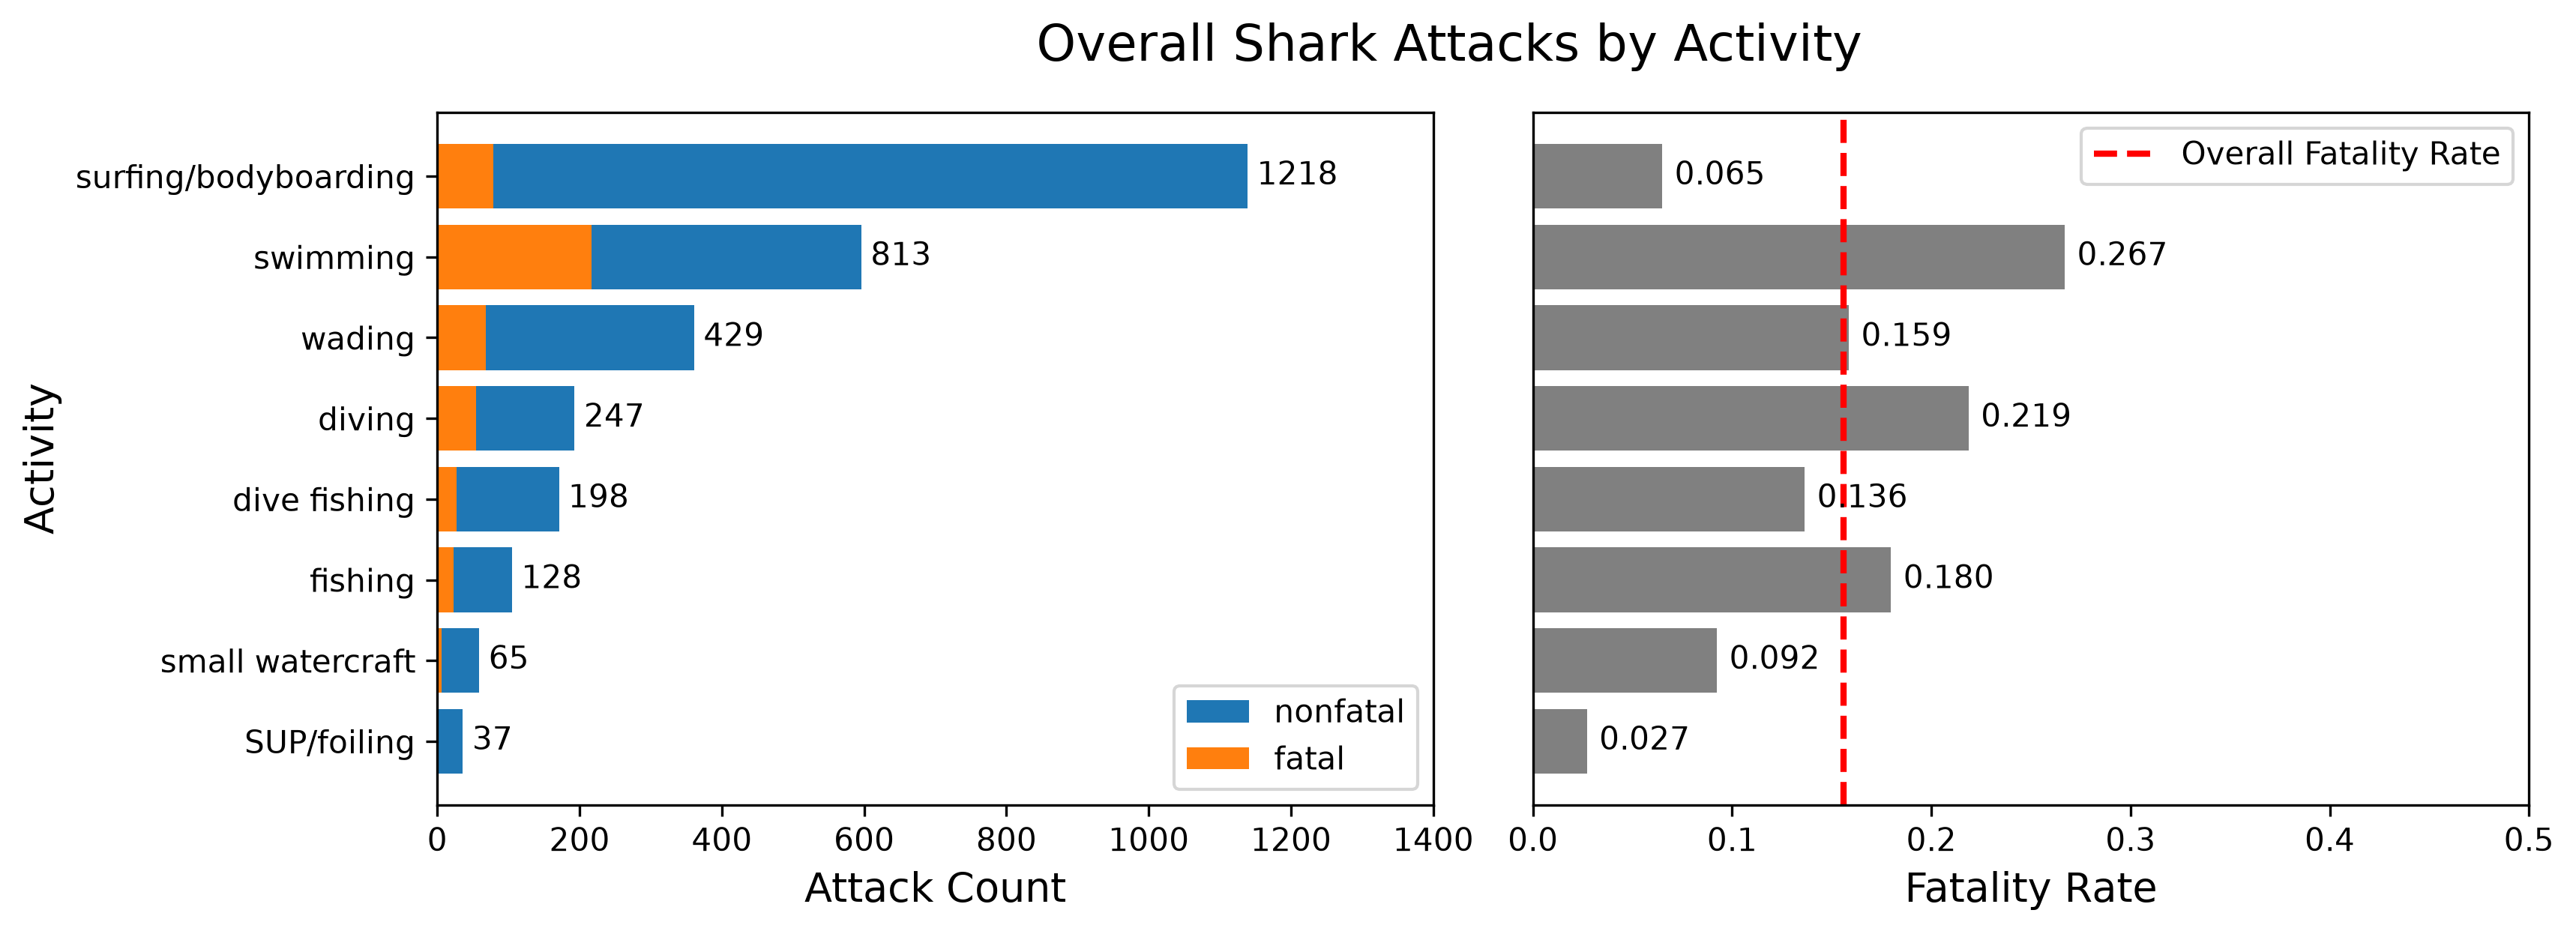
\includegraphics[width=1\textwidth,height=\textheight]{images/fatrate_plots_activity.png}

}

\caption{\label{fig-1}Shark attack counts and fatality rates by
activity}

\end{figure}%

If activity were to have no effect on fatality rate, one would expect
the fatality rate of each activity to be around the overall fatality
rate. Figure 1 shows that this is not the case. This is confirmed by a
chi-square test for independence that results in a p-value of less than
\(1.2 \times 10^{-33}\), suggesting activity and fatality are not
independent. While this is a strong result arising from a simple
associational analysis, we aim to go beyond this result to move towards
the asymptote of causality and attempt to quantify the causal effect of
activity. This begins with identifying some possible confounding
variables.

\paragraph{Analysis of species}\label{analysis-of-species}

The first possible confounding variable we analyze is species, the
results of the same analysis performed for activity in relation to
fatality rates are shown in Figure 2.

\begin{figure}

\centering{

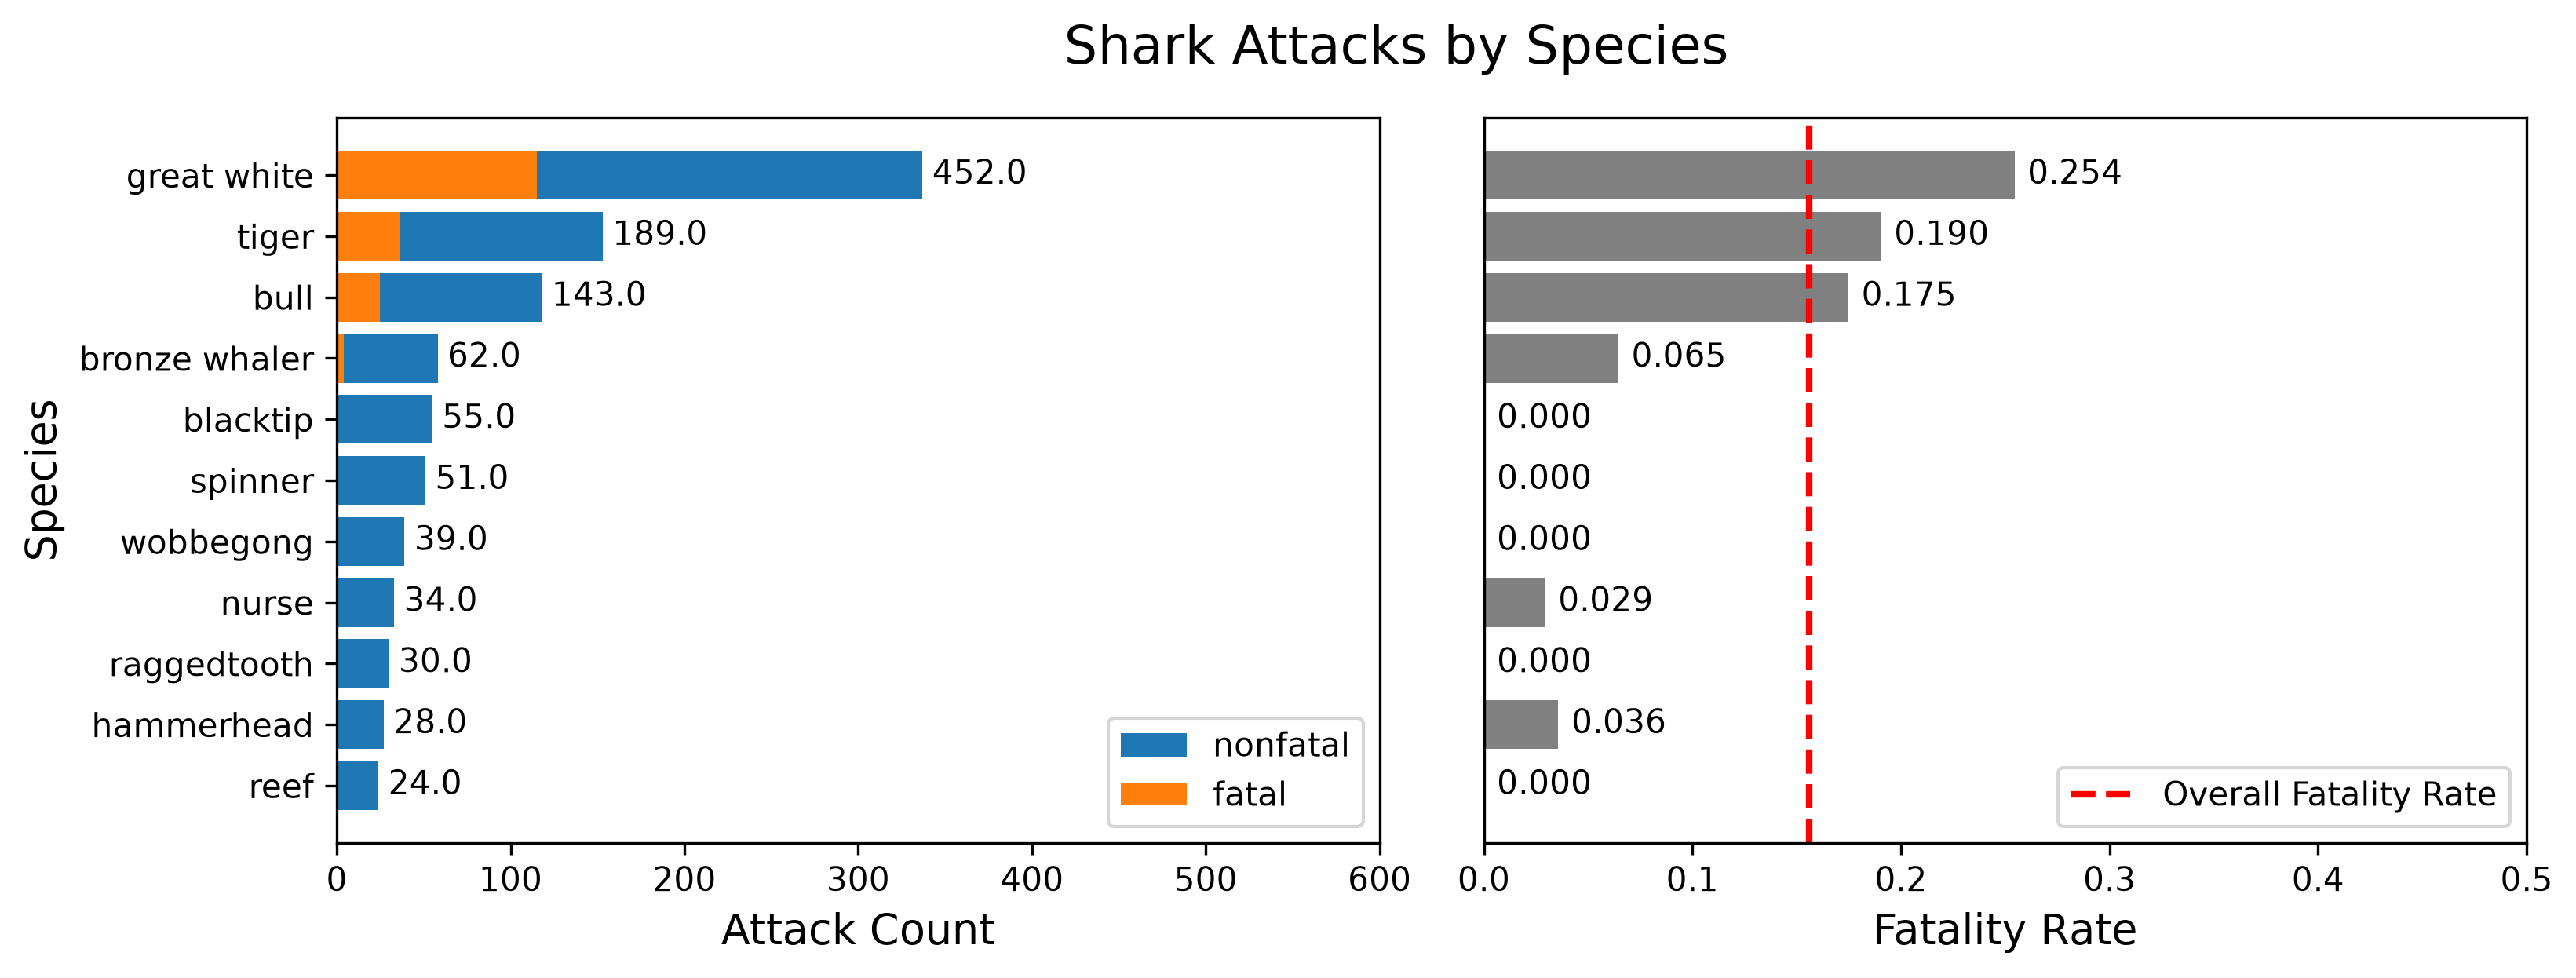
\includegraphics[width=1\textwidth,height=\textheight]{images/fatrate_plots_species.png}

}

\caption{\label{fig-2}Shark attack counts and fatality rates by species}

\end{figure}%

Species appears to have a strong affect on survivability when compared
to activity. With some species such as blacktip and spinner sharks
having no recorded fatal attacks in this subset of the dataset. On the
other hand, the fatality rate of attacks by great whites (25.4\%) is
well above the overall fatality rate of 15.6\%. A chi-square test
between species and fatality yields a p-value less than
\(3.6 \times 10^{-12}\), further suggesting the two variables are not
independent.

\paragraph{Analysis of season}\label{analysis-of-season}

Next, we take a look at shark attacks by season in Figure 3.

\begin{figure}

\centering{

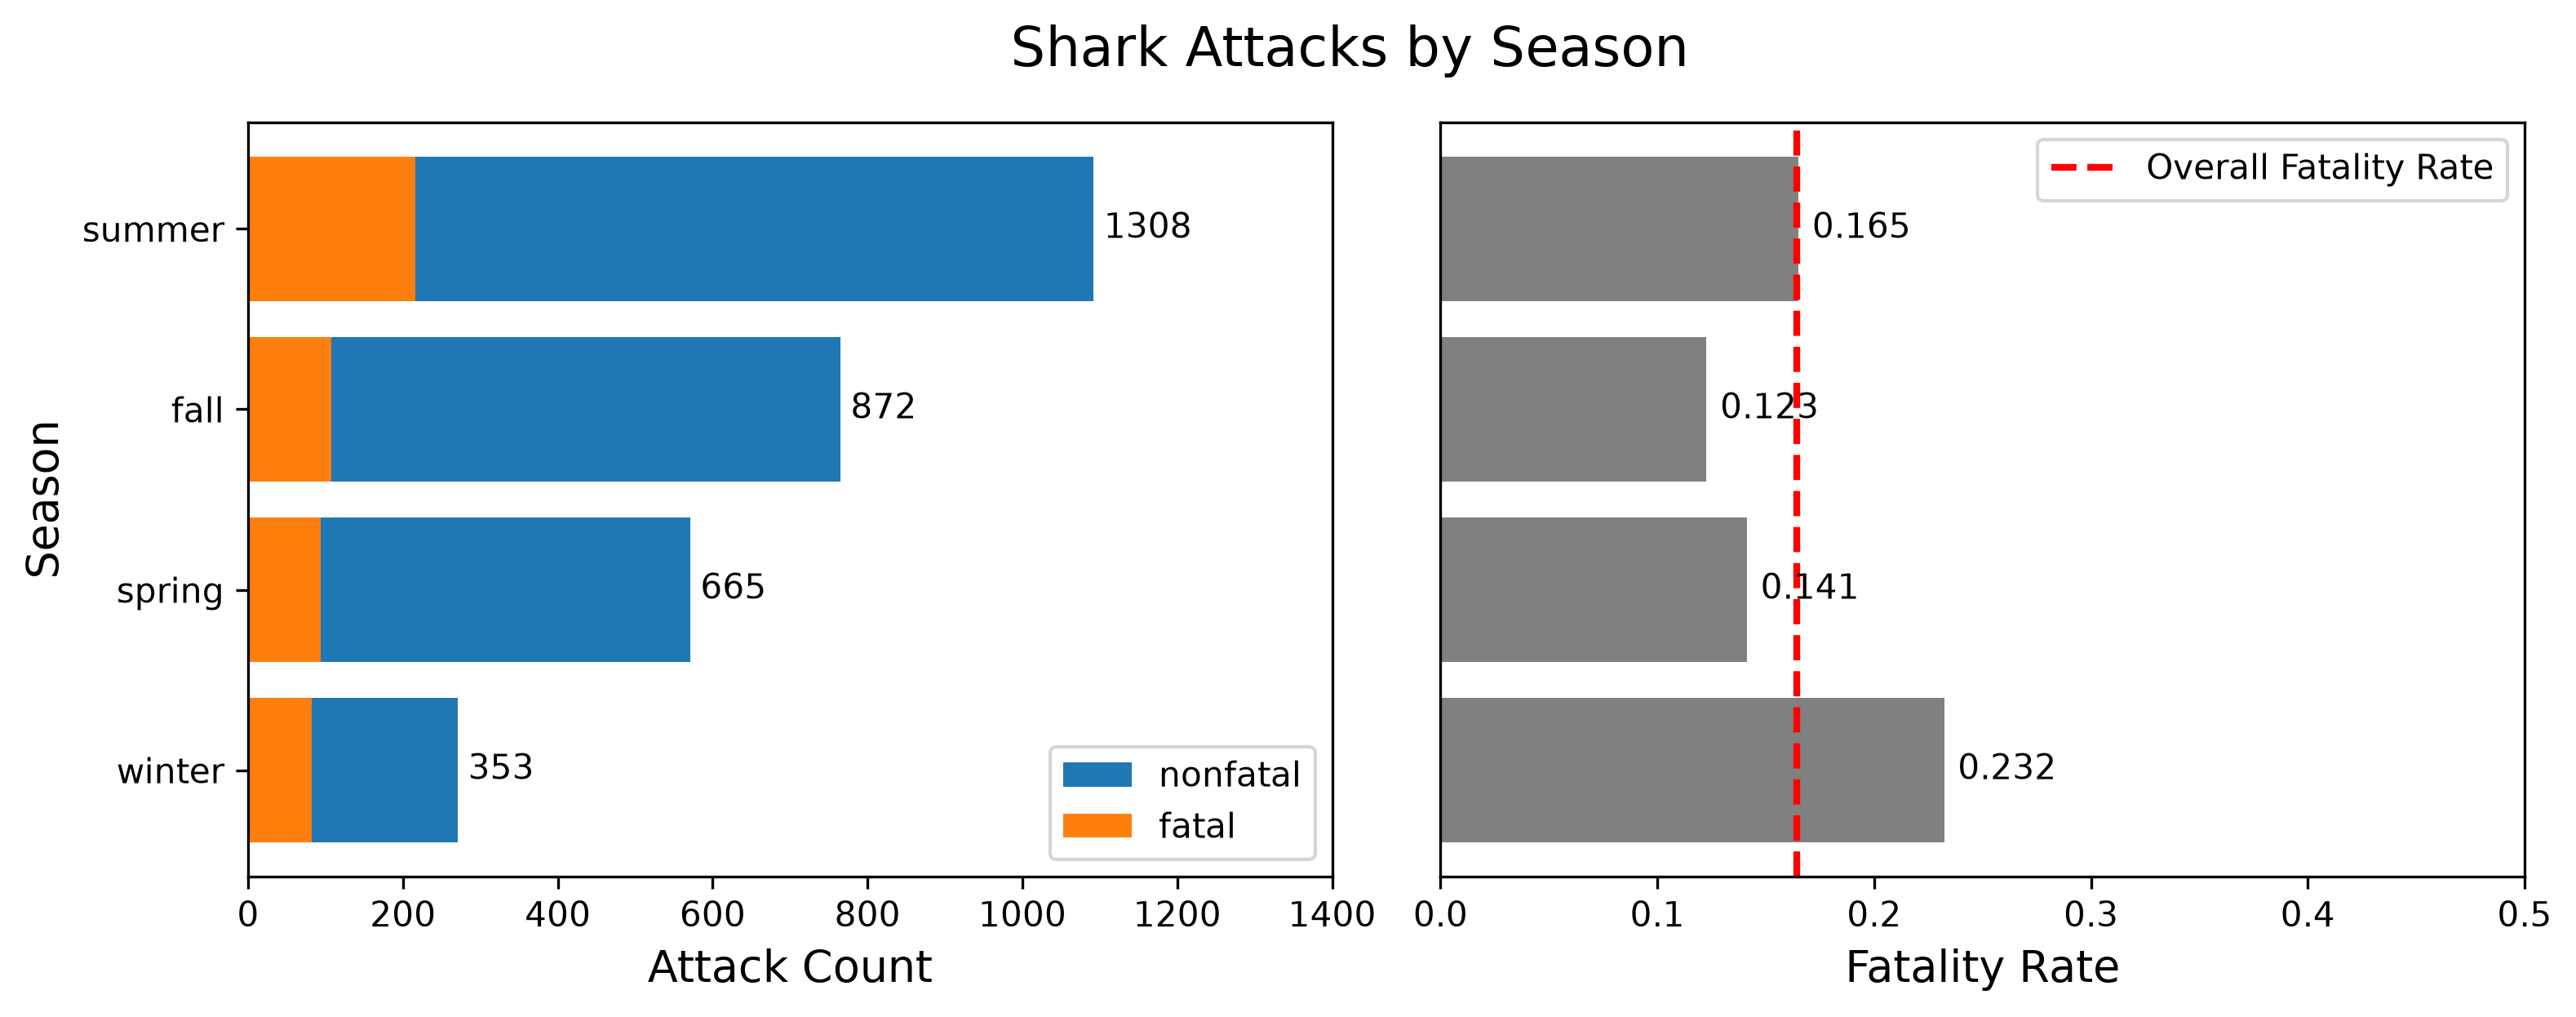
\includegraphics[width=1\textwidth,height=\textheight]{images/fatrate_plots_season.png}

}

\caption{\label{fig-3}Shark attack counts and fatality rates by state}

\end{figure}%

These results show that despite a significantly lower number of attacks,
winter has the highest fatality rate of all seasons at 23.2\%. A
chi-square test between season and fatality rate suggests the two
variables are not independent (\textless{}\(2 \times 10^{-5}\)). There
could be several reasons for the fluctuation in fatality rate across the
seasons. One such possibility is which sharks are present close to shore
around people during each season. Juvenile sharks tend to spawn during
the warmer months in the Spring and Summer, which is also when more
people tend to seek the beach for recreation. These juveniles are small
and less likely to inflict the type of wound that could lead to a
fatality. On the other hand, due to migration patterns, larger sharks
may be present closer to shore in populated areas like California and
off the coast of Australia. These encounters tend to be deadlier, as
shown in Figure 2.

\paragraph{Analysis of location
(state)}\label{analysis-of-location-state}

As mentioned by Midway, Wagner, and Burgess (2019), a number of local
conditions affect the number of shark attacks and shark related deaths
in a given region. The conditions include the local population level and
the species of shark present. We take a look at shark attacks and
fatality rates by state in Figure 4.

\begin{figure}

\centering{

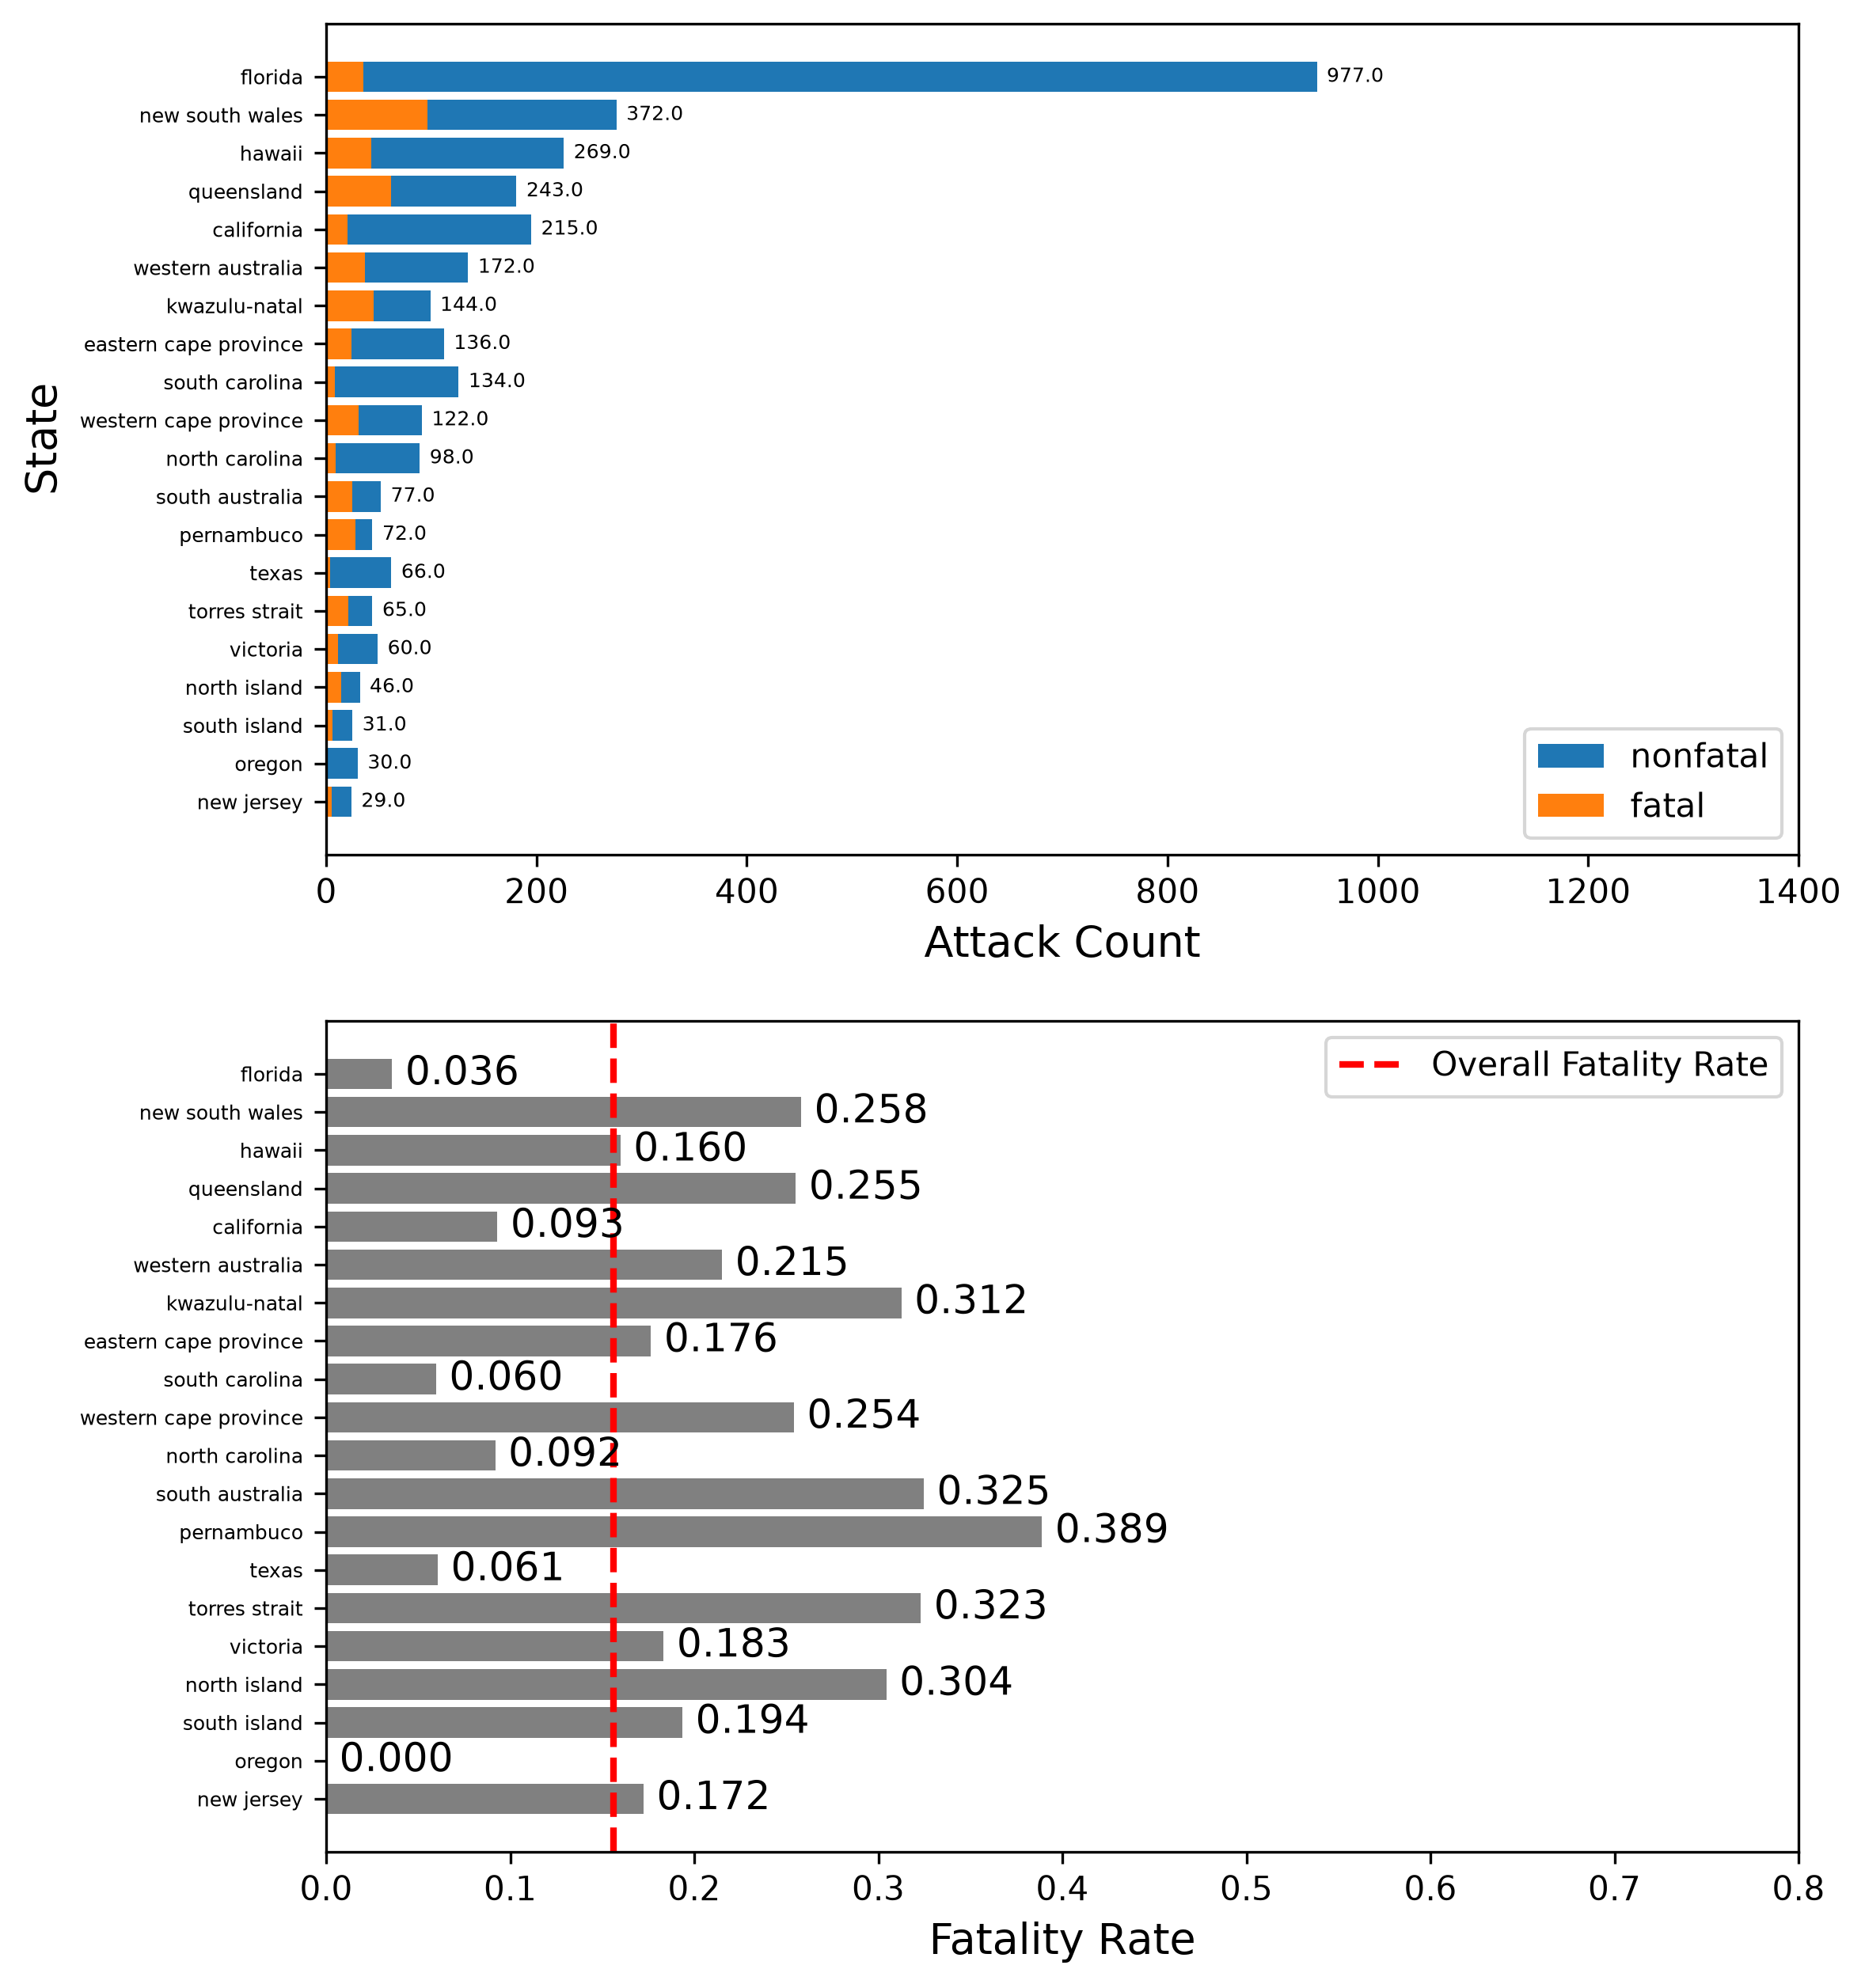
\includegraphics[width=1\textwidth,height=\textheight]{images/fatrate_plots_state.png}

}

\caption{\label{fig-4}Shark attack counts and fatality rates by state}

\end{figure}%

As can be seen in Figure 4, the fatality rates of each state in the
dataset tend to vary far from the overall fatality rate. Florida, which
has a disproportionately high rate of shark attacks, has a low fatality
rate of 3.6\%. The state with the second highest number of shark
attacks, New South Wales in eastern Australia, has a fatality rate of
25.8\%, which is well above the overall fatality rate of 15.6\%. State
and fatality rate are shown not to be independent with a chi-square test
that yields a p-value of less than \(5.5 \times 10^{-51}\). This
disparity in fatality rates can likely be explained by the different
species present in each state. Florida features predominantly small
shark species such as bull sharks, while Australia is known for its
larger population of great white sharks. This idea will be explored
further in subsequent sections.

\subsubsection{Exploring relationships between confounding variables and
activity}\label{exploring-relationships-between-confounding-variables-and-activity}

\begin{itemize}
\tightlist
\item
  include contingency tables
\item
  compare stats for different species/states/seasons
\end{itemize}

While the previous section focused on relationships between the
confounding variables we have identified (location, season, and species)
and fatality rates, this section focuses on relationships among
confounding variables and activity. This will be important when
constructing our probabilistic graphical model in the subsequent
sections. By understanding how the confounding variables interact with
activity, we can begin to construct pathways of causality through these
confounders to the probability of fatality.

\paragraph{Activity and season}\label{activity-and-season}

It seems reasonable to guess that the season can influence the activity
being performed in which a shark attack took place. For example, winter
typically comes with stronger storms which generate larger waves. These
conditions are great for surfers, less so for swimmers (especially when
also factoring in the cold). We look to figure 5 to see if this
assumption has any merit.

\begin{figure}

\centering{

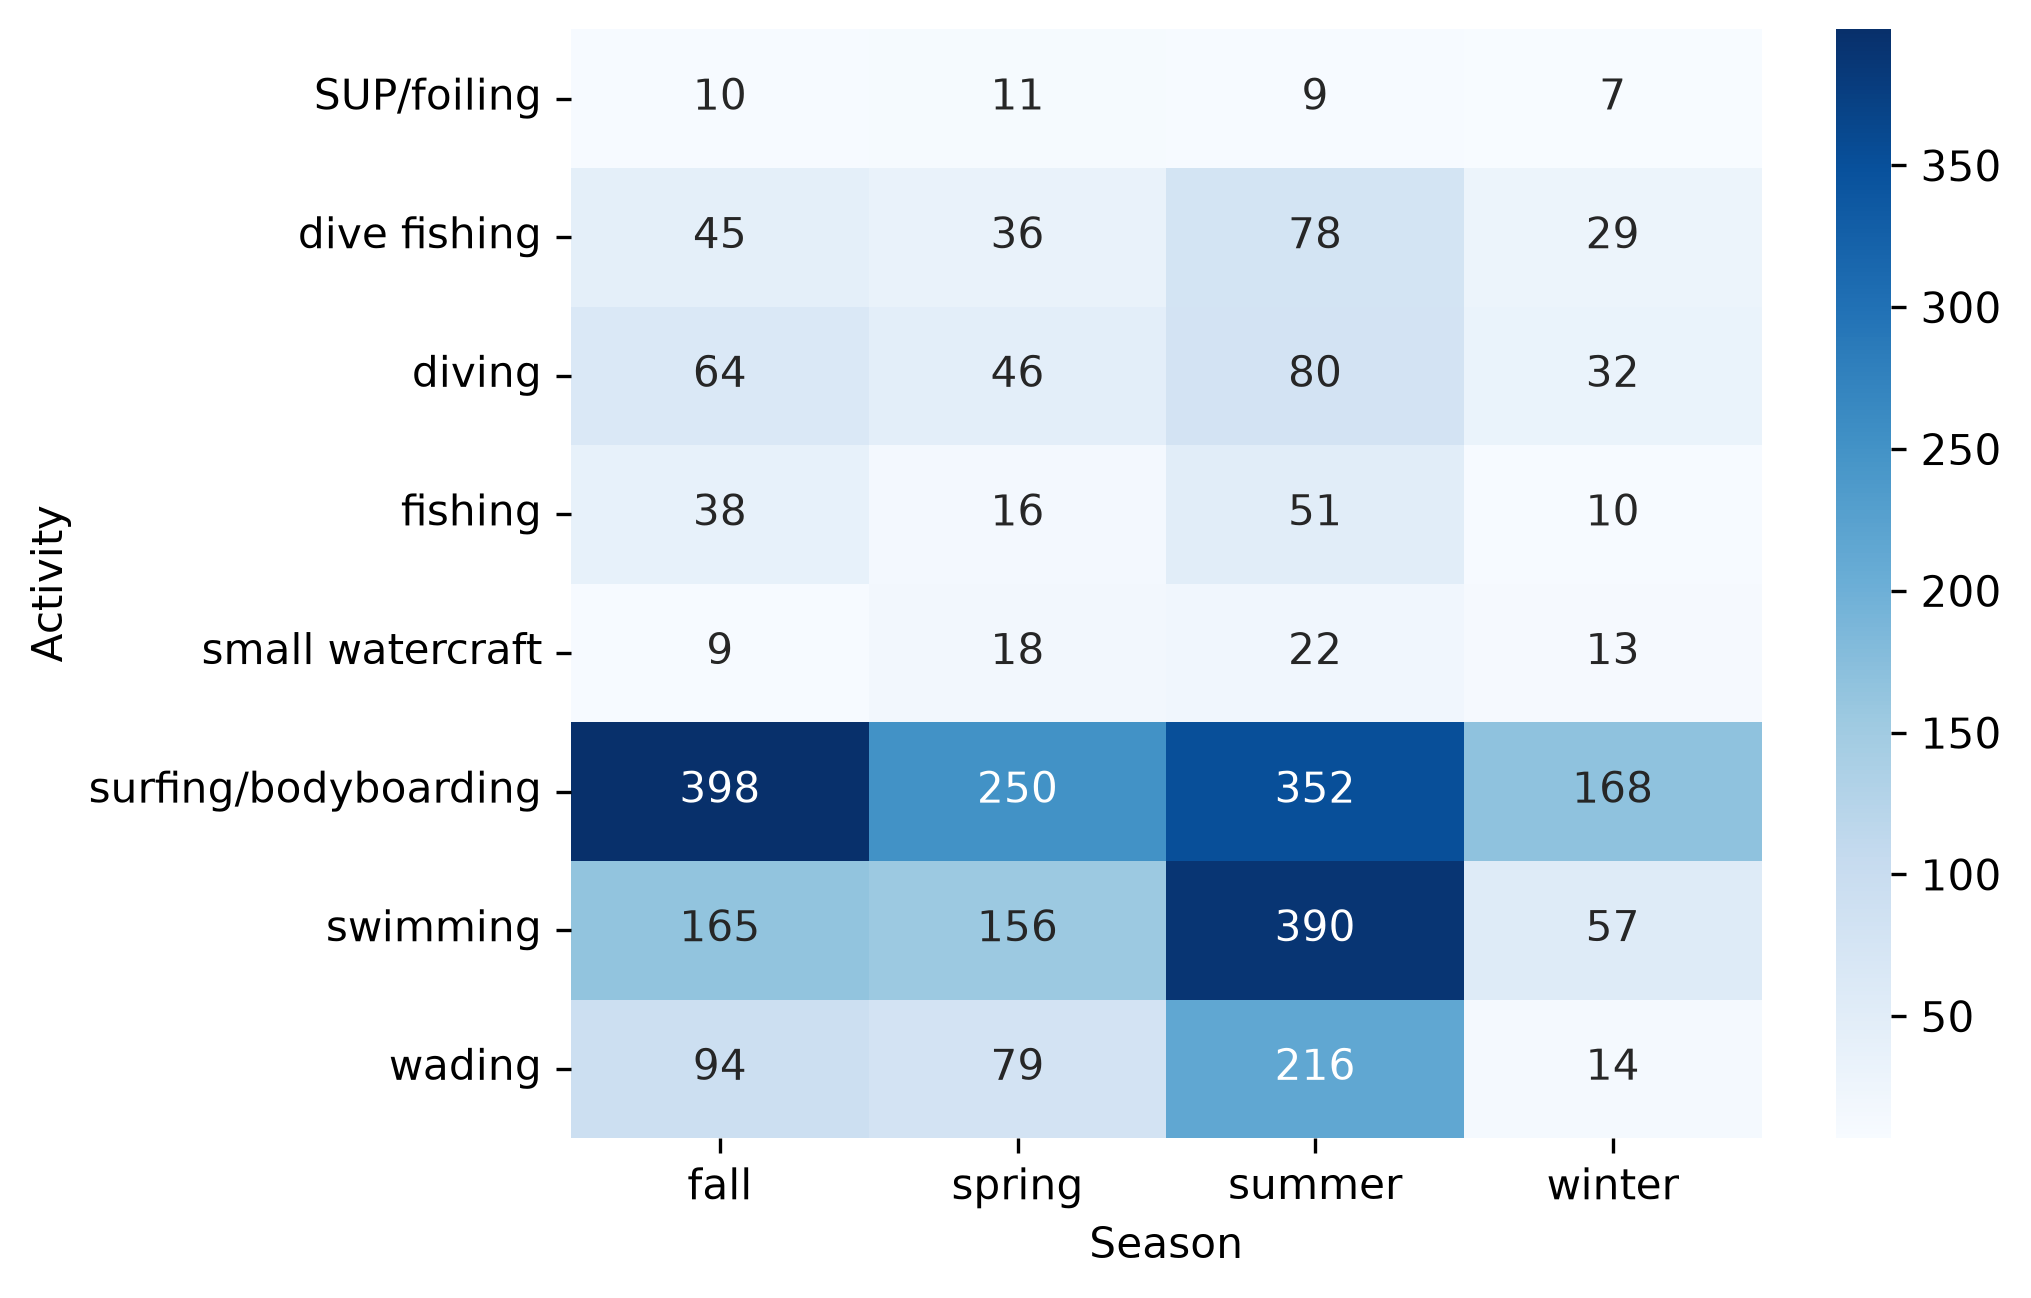
\includegraphics[width=0.6\textwidth,height=\textheight]{images/activity_season.png}

}

\caption{\label{fig-5}Contingency plot comparing activity and season of
shark attacks}

\end{figure}%

Figure 5 indeed shows fluctuations in each activity by season as well as
changes in their proportions in relation to each other by season. Winter
months bring cold weather and cold water, and thus see precipitous drops
in swimming and wading. During these months, someone who is attacked is
more likely to be surfing than swimming/wading. This trend flips during
the summer, in which more people come to the beach for casual
recreation, bringing a spike in attacks on swimmers and waders relative
to surfers.

\paragraph{Activity and location}\label{activity-and-location}

\begin{figure}

\centering{

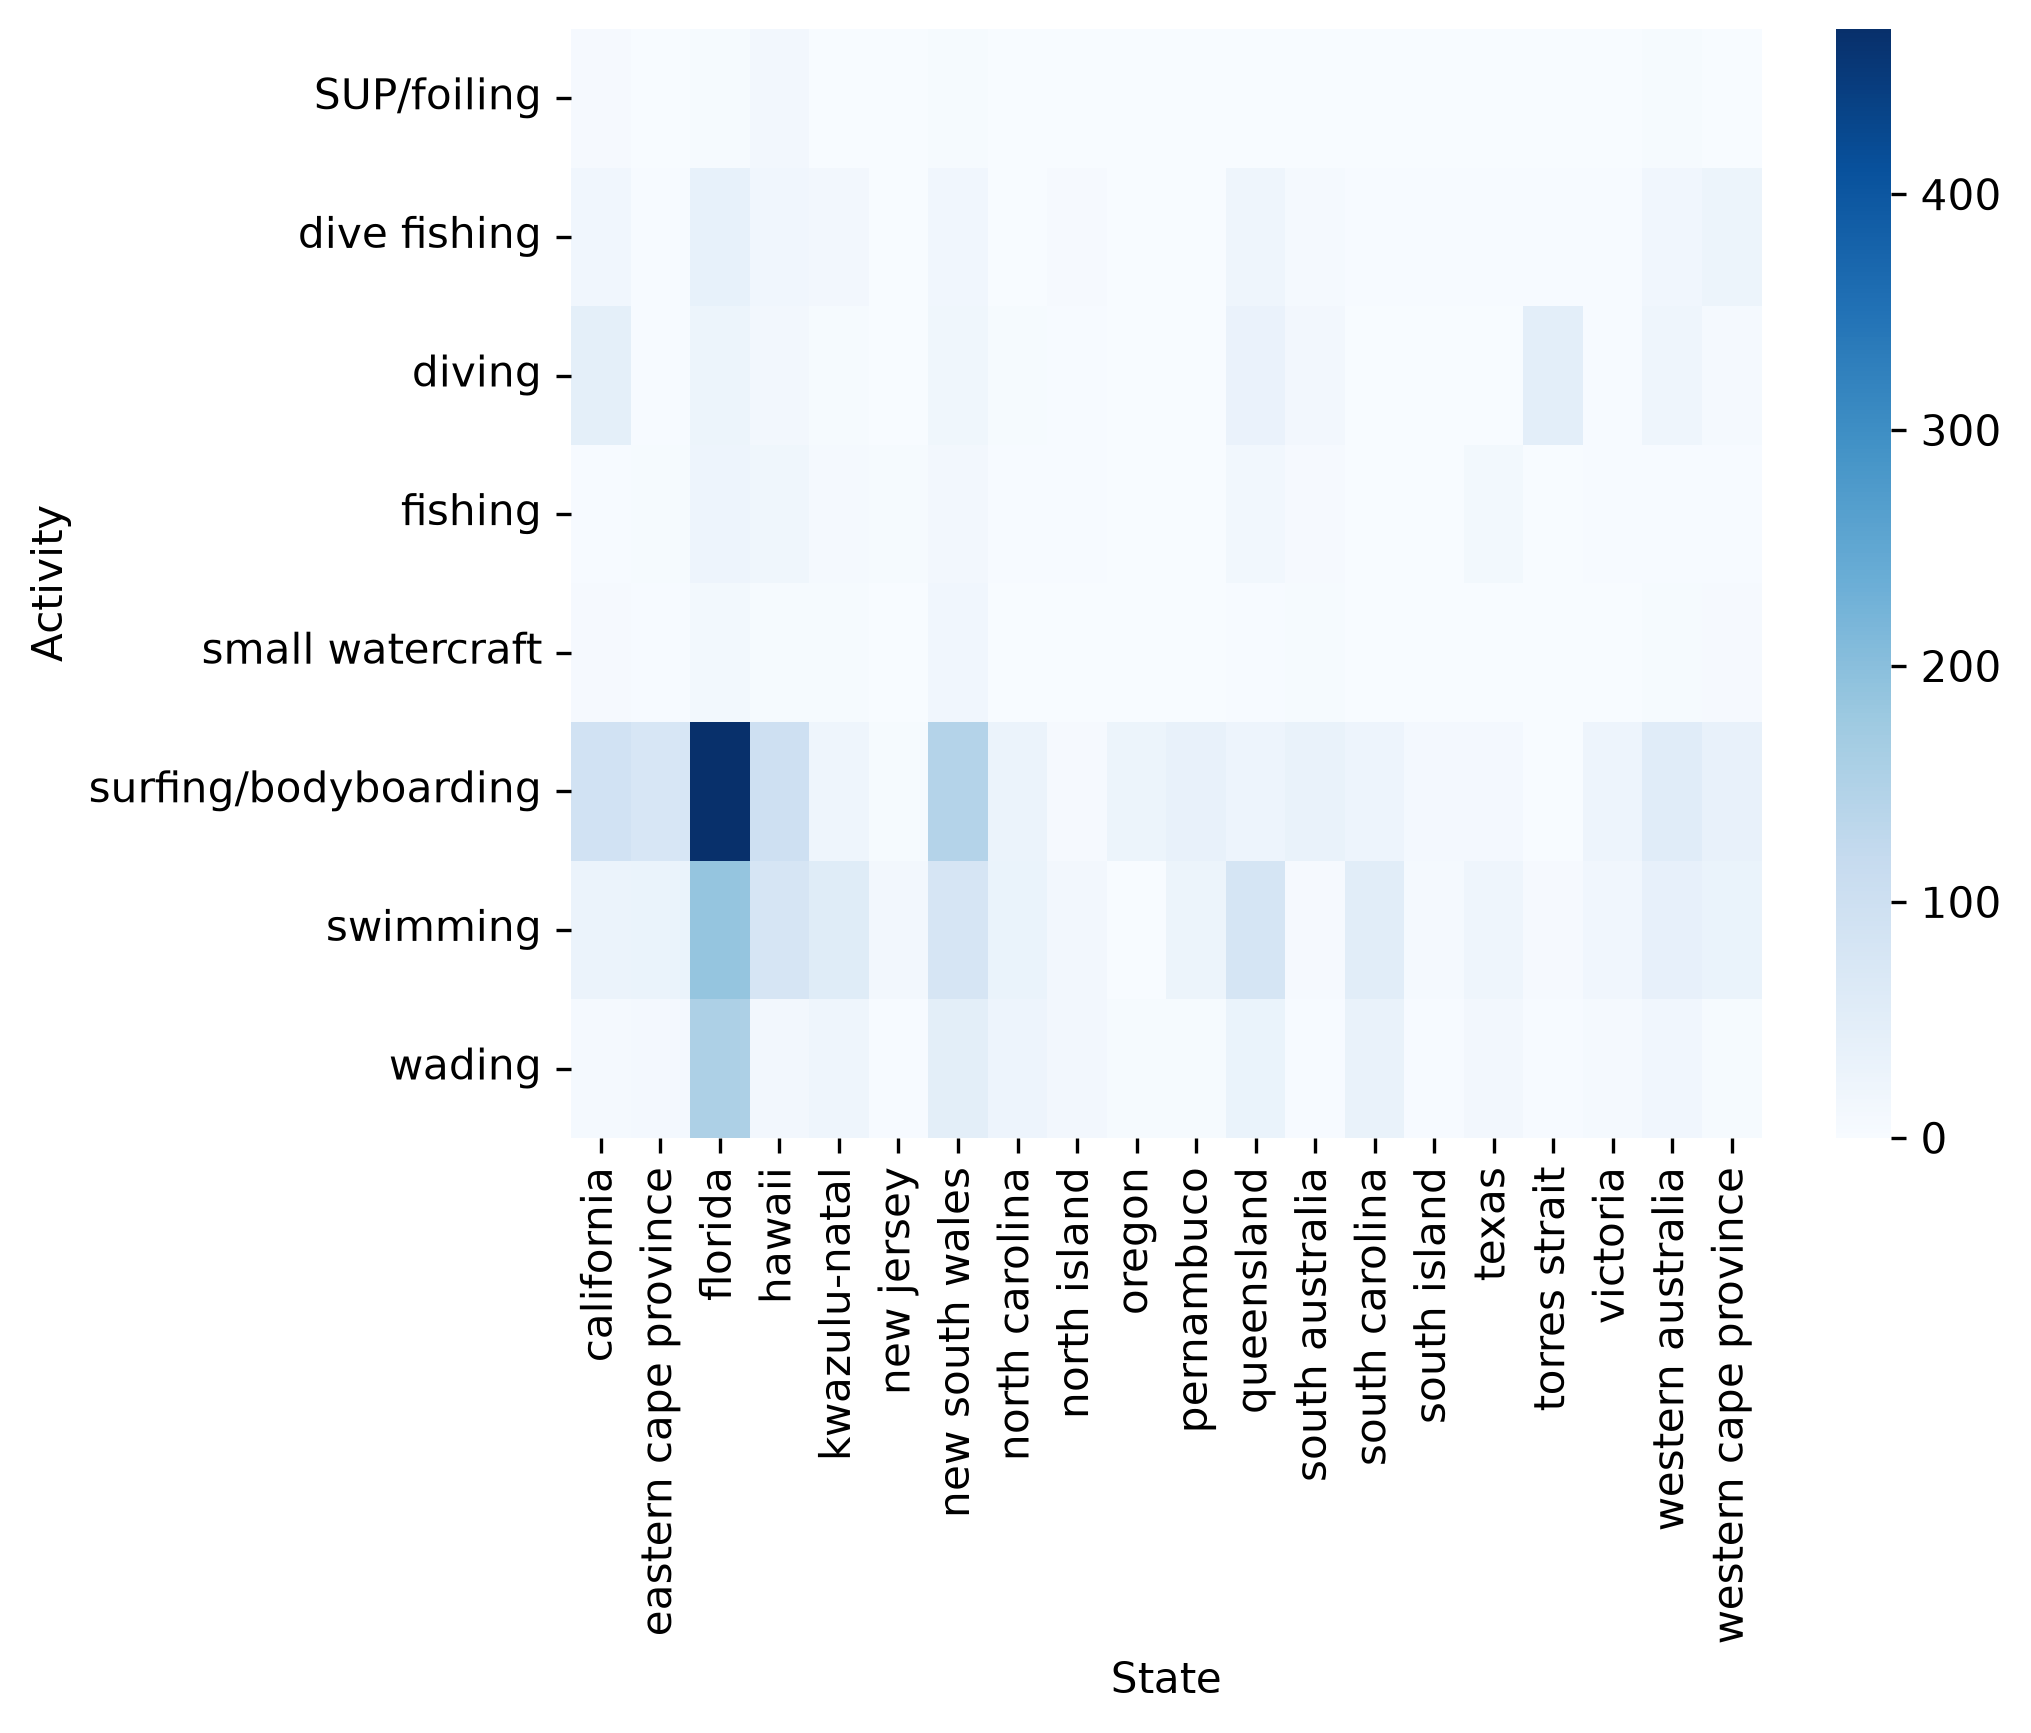
\includegraphics[width=0.6\textwidth,height=\textheight]{images/activity_state.png}

}

\caption{\label{fig-6}Heat map comparing activity and state in which
attack took place}

\end{figure}%

Figure 6 shows counts of attacks based on activity and state. The
popularity of activities varies by state, with surfing being the most
popular in some states and swimming being the most popular in others.
This could be due to several factors, such as the local culture and the
conditions for each activity in the region.

\paragraph{Season and species}\label{season-and-species}

\begin{figure}

\centering{

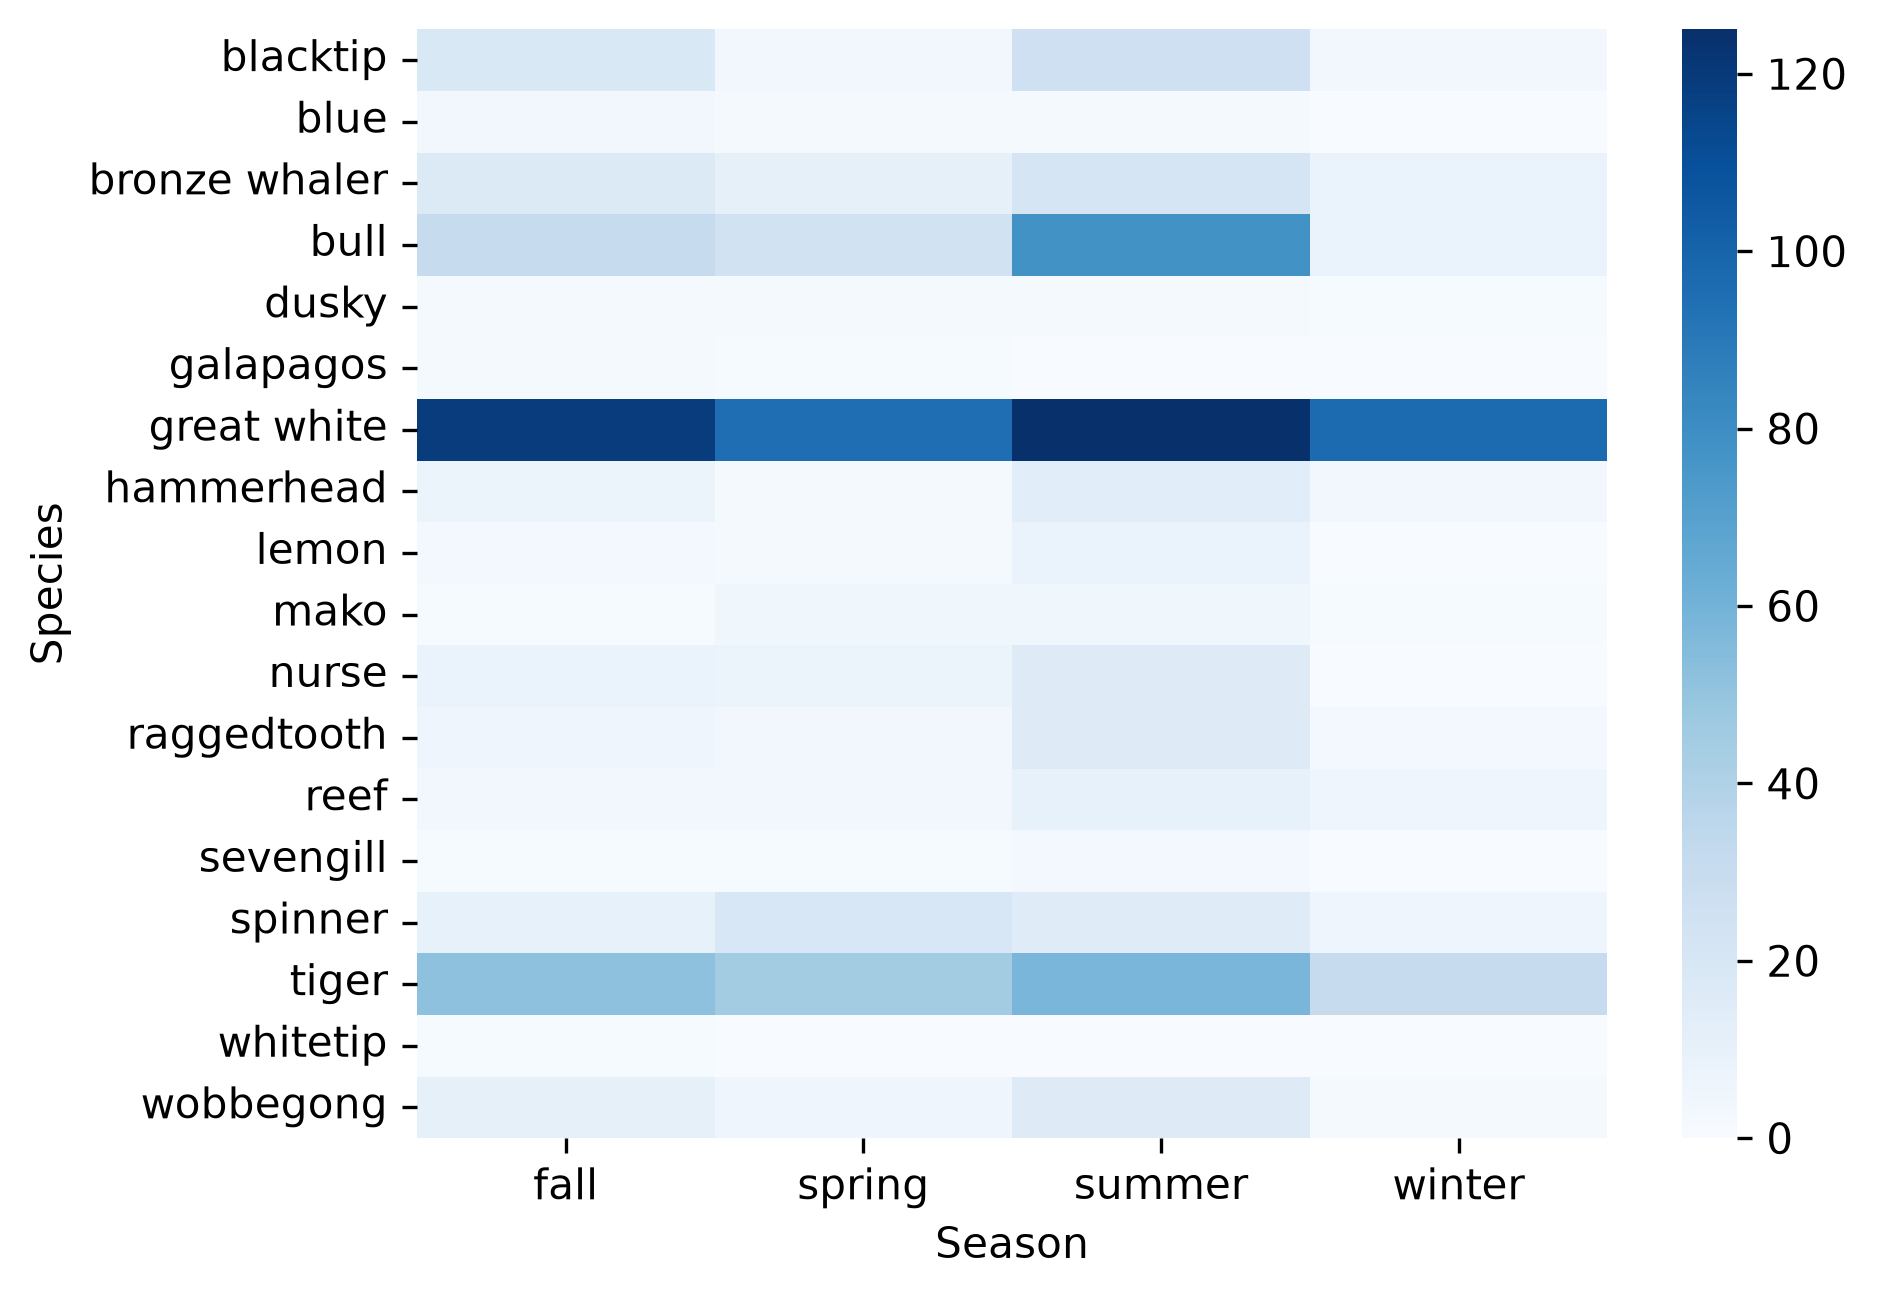
\includegraphics[width=0.6\textwidth,height=\textheight]{images/season_species.png}

}

\caption{\label{fig-7}Heat map comparing species and season in which
attack took place}

\end{figure}%

The heatmap in Figure 7 shows fluctuations in attacks by different
species across seasons. For nearly all species, more attacks occur in
the fall and summer months. Bull sharks stand out, as a higher
proportion of bull shark attacks occur during the summer months when
compared to other species in relation to other seasons.

\paragraph{Location and species}\label{location-and-species}

\begin{figure}

\centering{

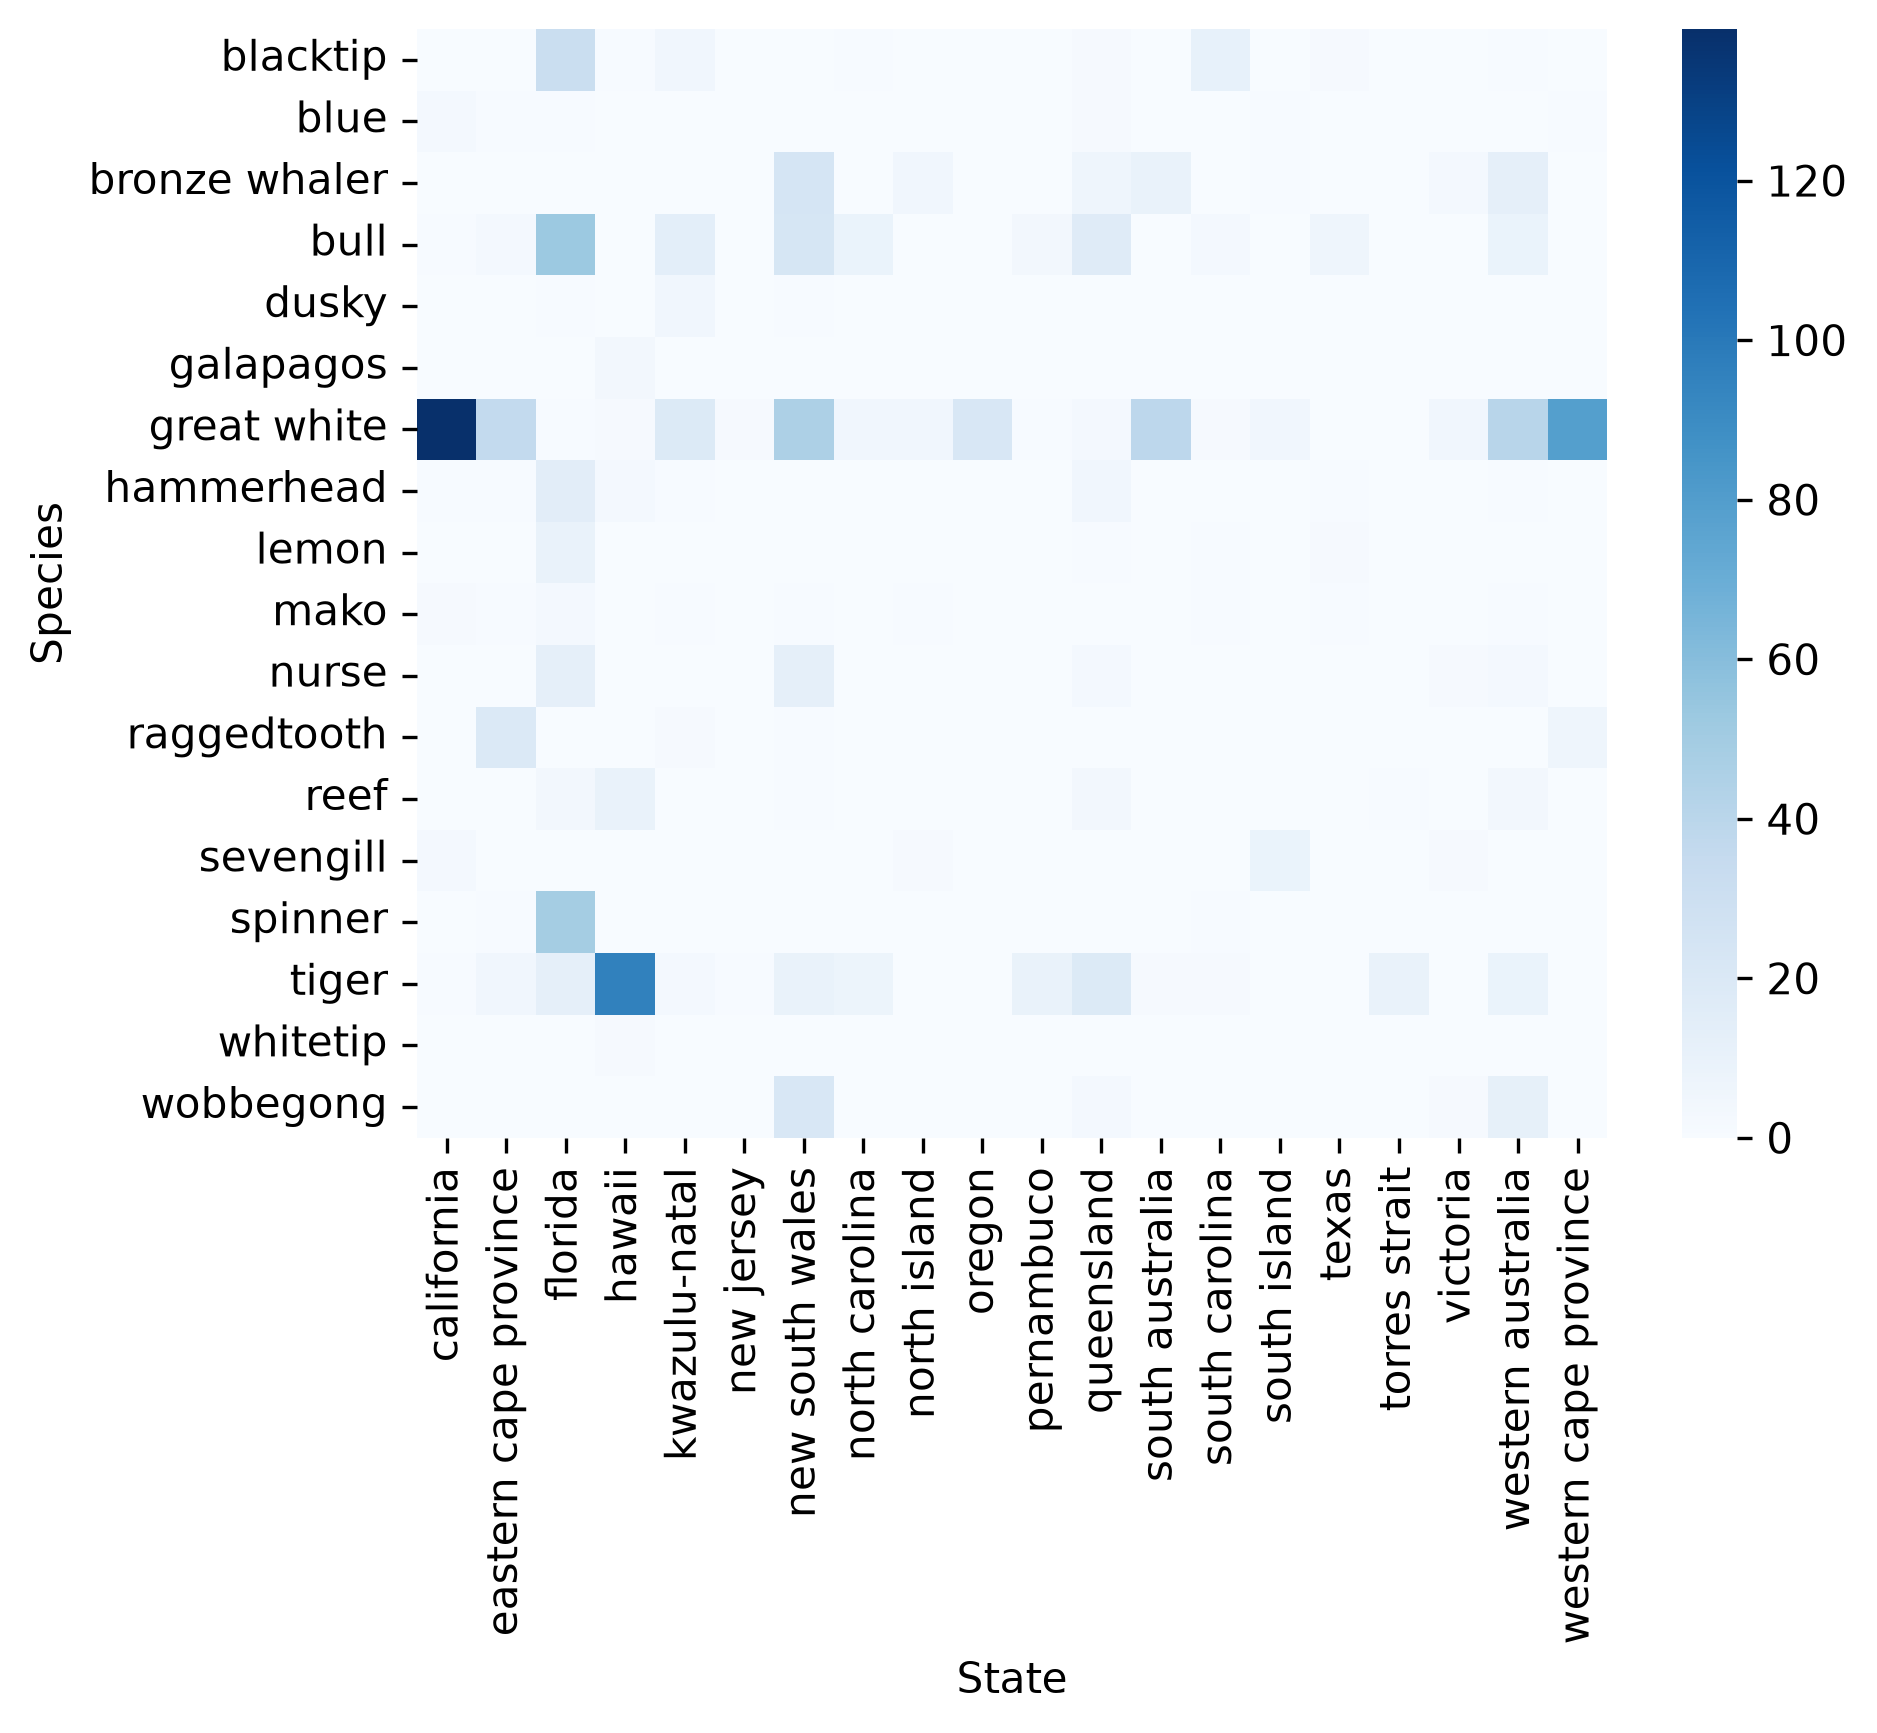
\includegraphics[width=0.6\textwidth,height=\textheight]{images/state_species.png}

}

\caption{\label{fig-8}Heat map comparing species and state in which
attack took place}

\end{figure}%

Figure 8 demonstrates the differences in distribution of shark species
across regions (states). California stands out for having nearly every
single attack be due to a great white shark. Other states, such as
Florida, see a wider variety of shark species involved in attacks that
are typically associated with lower death rates. This helps explain the
disparity in fatality rates across states shown in section 2.2.4. This
plot shows a strong relationship between state and the shark species
present during attacks.

\subsection{Moving toward causality: how confounders influence treatment
effect}\label{sec-3}

For the purposes of this study, we would like to investigate the effect
confounding variables may have on the associational correlation we
observed between activity and fatality rate. The confounding effect of
location is made clear in Figure 9 below.

\begin{figure}

\centering{

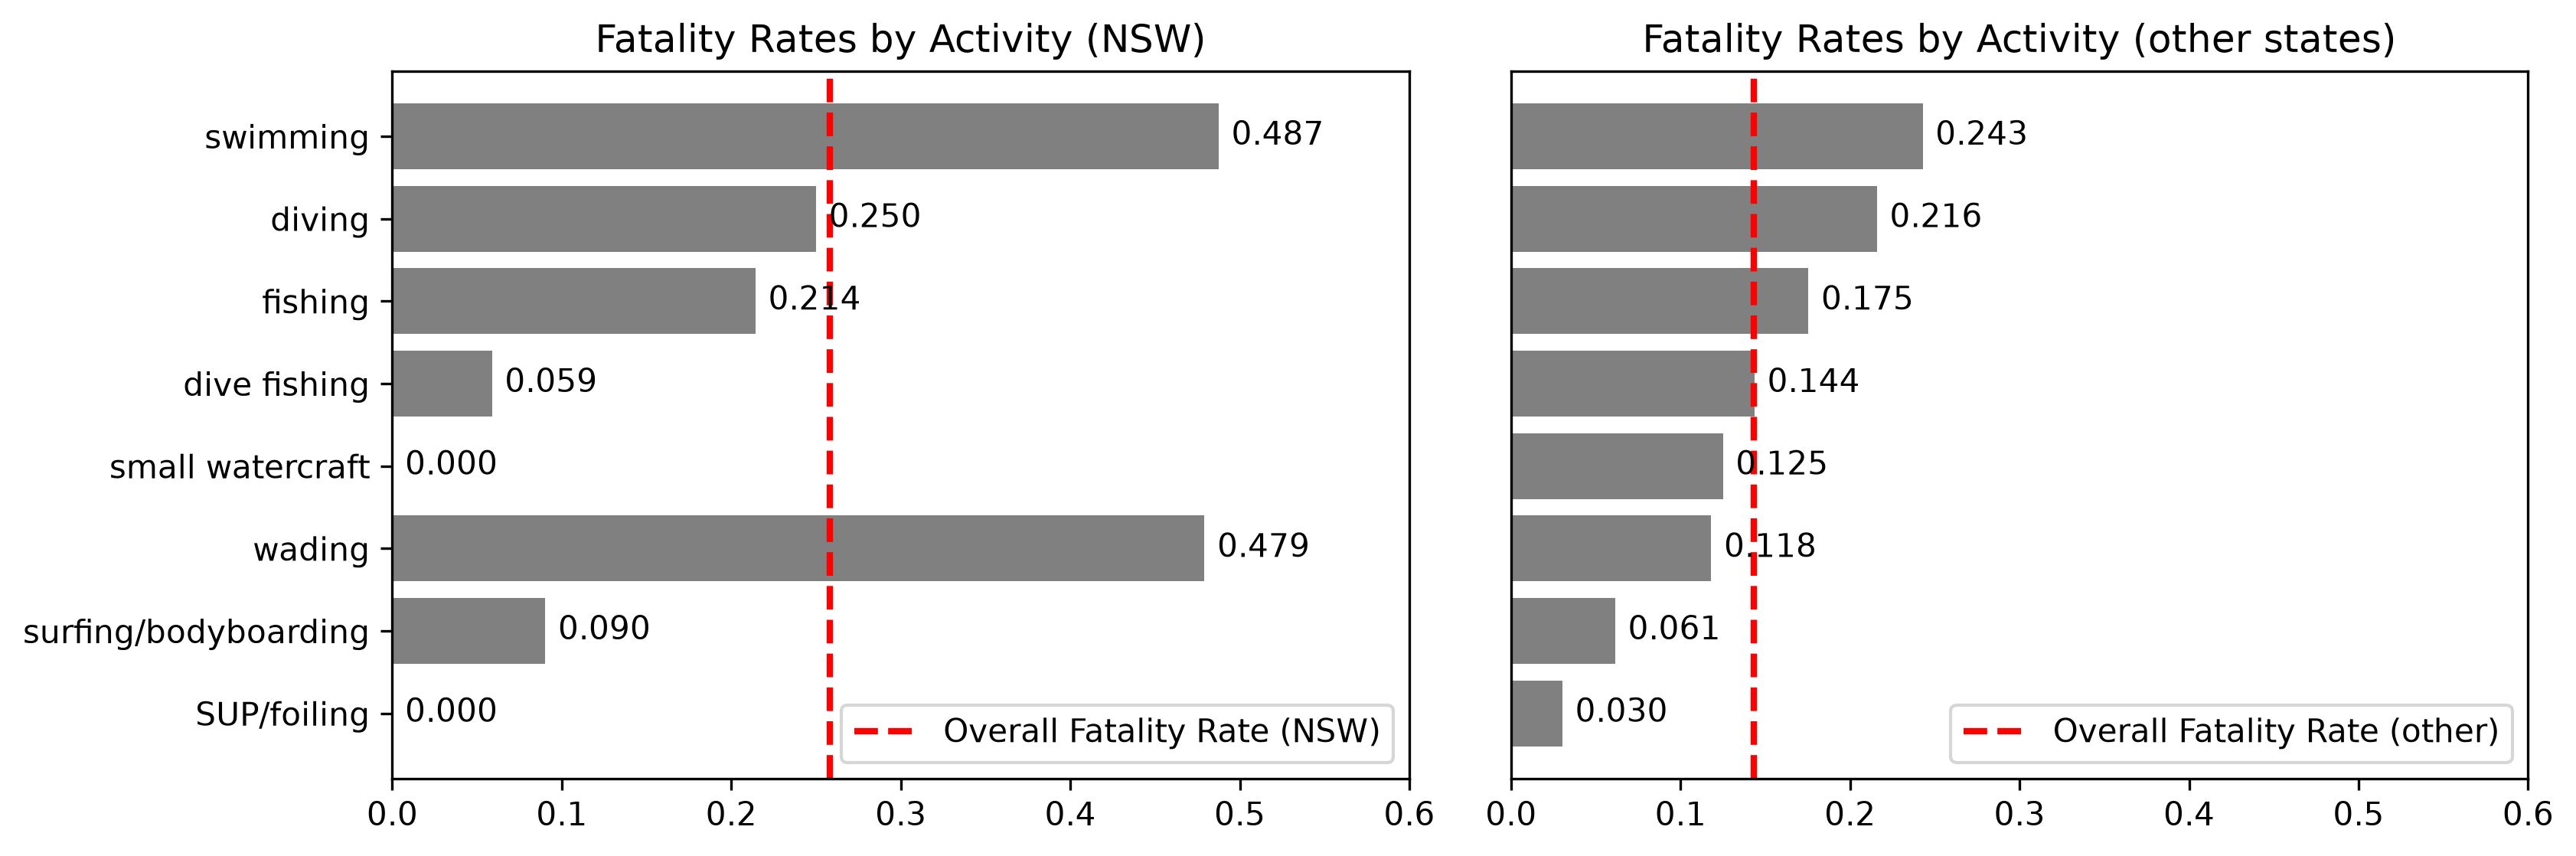
\includegraphics[width=1\textwidth,height=\textheight]{images/nsw_vs_other.png}

}

\caption{\label{fig-9}Comparing fatality rates by activity in New South
Wales vs all other states}

\end{figure}%

The overall fatality rate in New South Wales is 25.8\%, while the
overall fatality rate across all other states in our analysis is 14.3\%.
Fatality rates across activities are generally higher across the board
in New South Wales. The fatality rate of attacks on swimmers in New
South Wales is more than twice that of all other states when combined.
More importantly, the relative danger of each activity compared to other
activities is different in New South Wales. This is most obvious when
looking at the fatality of wading. Attacks on people in shallow water in
New South Wales are dramatically higher than other activities except for
swimming. This is very different from the rest of the population as a
whole, where wading tends to have a lower fatality rate than the
majority of other activities.

These results show that activity alone does not adequately capture the
risk of death when attacked by a shark, and the location of the attack
is indeed a confounding variable that must be accounted for when trying
to measure the causal effect of activity on shark attack survivability

\subsection{Modeling with a probablistic graphical model}\label{sec-4}

\begin{figure}

\centering{

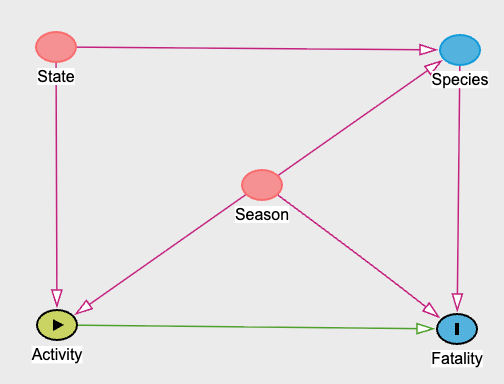
\includegraphics[width=0.4\textwidth,height=\textheight]{images/dag.png}

}

\caption{\label{fig-10}Probablistic graphical model depicting potential
data generating process}

\end{figure}%

The above model depicts a proposed data generating process with each of
the variables we have covered so far in our analysis. The activity at
the time of the attack is considered the treatment effect, while whether
the attack resulted in a fatality is our outcome of interest. The
purpose of this model is to give a clear idea of which backdoor paths
must be closed to isolate the effect of activity on fatality.

\subsubsection{Next steps}\label{next-steps}

\textbf{Test Validity of PGM:} This PGM implies multiple conditional
independencies. * activity independent of species when conditioned on
season and state * fatality independent of state when conditioned on
activity, season, and species * state independent of season These
conditional independencies should be tested in order to determine if
this PGM is invalid as proposed

\textbf{Model PGM in PyMC:} Once those conditional independencies have
been tested, a model of this data generating process should be created
in PyMC to enable the ability to perform do-calculus to isolate the
effect of activity. I tried (with limited success) to implement a
discrete choice and random utility model in PyMC to model an individuals
choice of activity. When fully implemented, such a model will enable
further analysis to determine the causal effect of activity on fatality.

\subsection{References}\label{references}

\phantomsection\label{refs}
\begin{CSLReferences}{1}{0}
\bibitem[\citeproctext]{ref-midway2019trends}
Midway, Stephen R, Tyler Wagner, and George H Burgess. 2019. {``Trends
in Global Shark Attacks.''} \emph{PloS One} 14 (2): e0211049.

\bibitem[\citeproctext]{ref-neff2015jaws}
Neff, Christopher. 2015. {``The Jaws Effect: How Movie Narratives Are
Used to Influence Policy Responses to Shark Bites in Western
Australia.''} \emph{Australian Journal of Political Science} 50 (1):
114--27.

\bibitem[\citeproctext]{ref-ricci2016shark}
Ricci, Joseph A, Christina R Vargas, Dhruv Singhal, and Bernard T Lee.
2016. {``Shark Attack-Related Injuries: Epidemiology and Implications
for Plastic Surgeons.''} \emph{Journal of Plastic, Reconstructive \&
Aesthetic Surgery} 69 (1): 108--14.

\bibitem[\citeproctext]{ref-de2021factors}
Vasconcelos, Larissa Michelle Tenorio de, Halerrandro Gomes Borba,
Nelson Miguel Galindo Neto, Ana Carla Silva Alexandre, Juliana Lourenco
de Arajo Veras, and Silvia Elizabeth Gomes de Medeiros. 2021. {``Factors
Associated with Shark Attacks and Deaths: A Cross-Sectional Study.''}
\emph{Age} 3: 11--15.

\bibitem[\citeproctext]{ref-worm2013global}
Worm, Boris, Brendal Davis, Lisa Kettemer, Christine A Ward-Paige,
Demian Chapman, Michael R Heithaus, Steven T Kessel, and Samuel H
Gruber. 2013. {``Global Catches, Exploitation Rates, and Rebuilding
Options for Sharks.''} \emph{Marine Policy} 40: 194--204.

\end{CSLReferences}



\end{document}
